% Chapter 6

\chapter{Multi-lable Classification Methodology} % Write in your own chapter title
\label{Chapter6}
\lhead{Chapter 6. \emph{Methodology}}

\section{Artificial Dataset}

To demonstrate the approach, the dataset, named color detector, is created artificially. To each image, it has three labels for representing colour, $red$, $green$ and $blue$. If an image is red hue, it has a label for $red$ and label values of $green$ and $blue$ are negative. The representation of colour combination follows colour wheels. If an image has a hue close to $purple$, it has positive labels for $red$ and $blue$, and negative label for $green$, and so on.
\graphicspath{ {./Figures/} }
\begin{figure}[!htb]
\centering
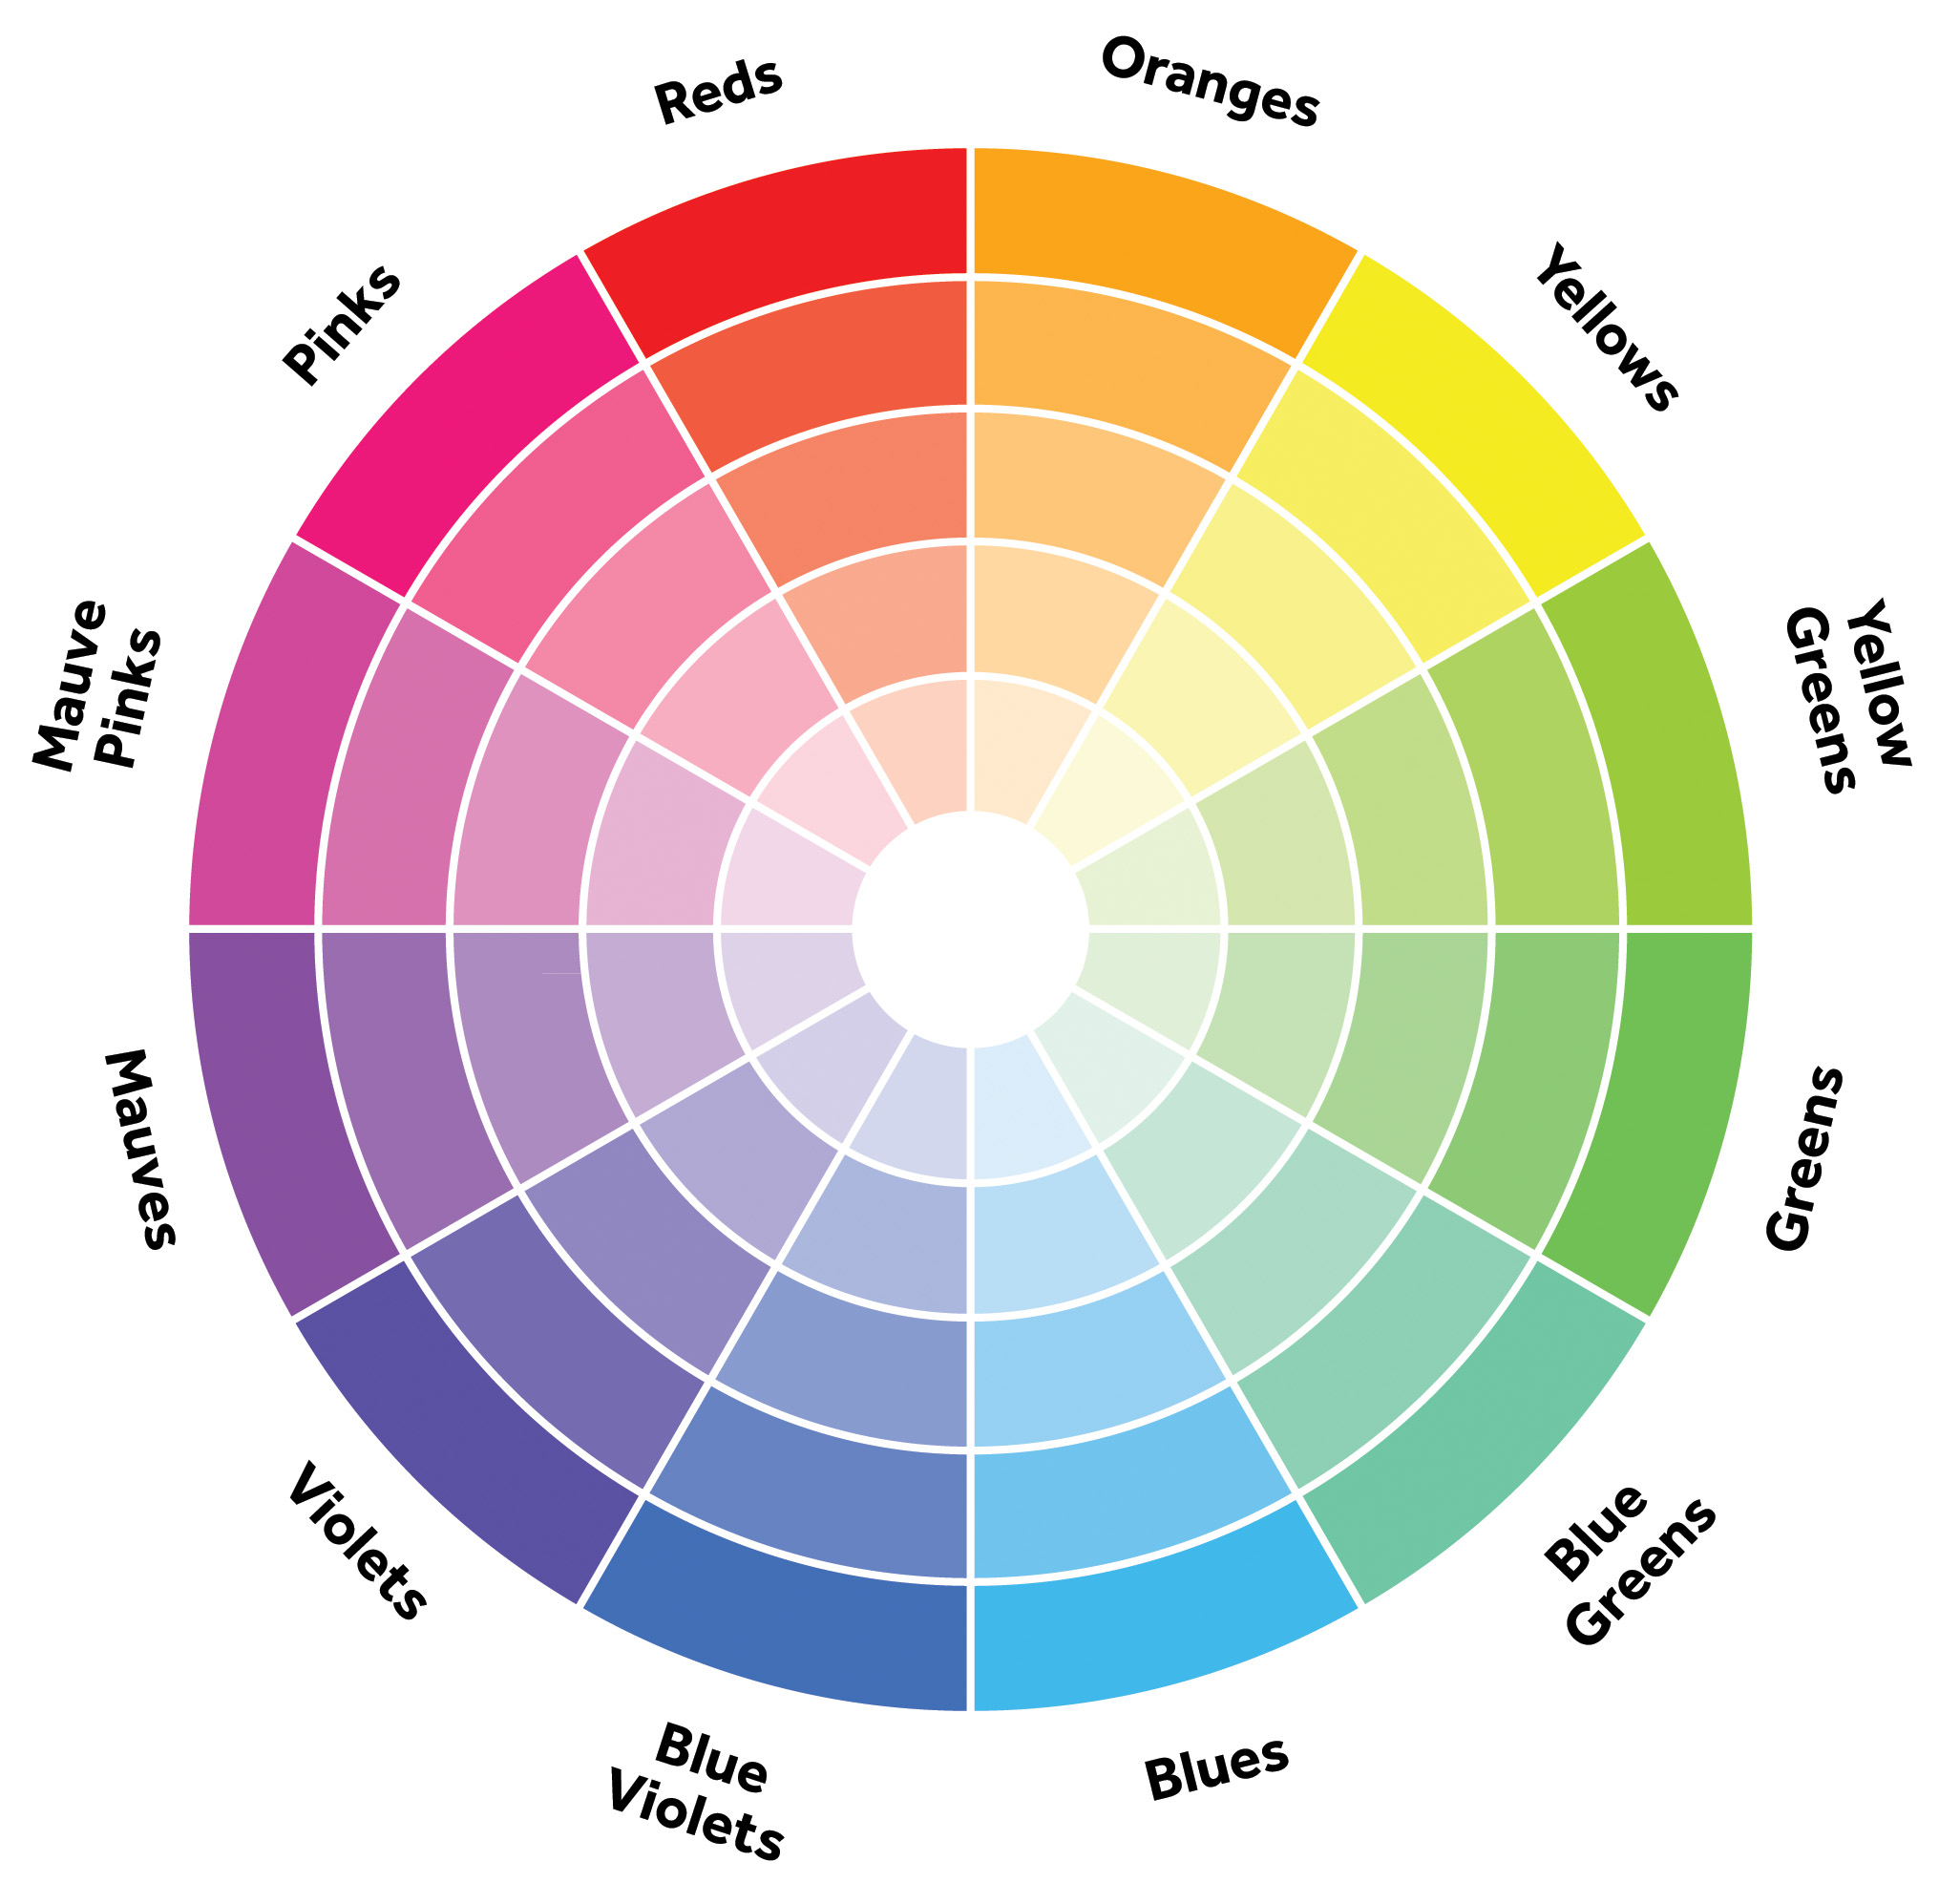
\includegraphics[scale=0.1]{color_wheel.jpg}
\caption{\label{fig:perceptron}Colour Wheel Diagram}
\end{figure}

For each sample $x_{i}$, it owns 3 labels ${y_{0},y_{1},y_{2}} y_{j} \in \{-1,1\}$ which represent $red$, $green$ and $blue$ respectively.

\subsection{Colour Generation}

To generate dataset artificially, we create $16x16$ size images and each image has $256$ pixels. For each pixel, we generate a random floating point number $h$ in the range $[0.0, 1.0)$ and use it as value for Hue via formulation.
\begin{equation}\label{eq:FormulationHue}
H = h + r * 0.4 - 0.2 (r \in [0.0,1.0))
\end{equation}
Where $r$ is another random floating point number. Then we generate 2 random floating point numbers as Saturation(S) and Value(V) values. We transform HSV values to RGB values and time $255$ for each pixel. Repeating the steps, we can get a $256$ pixels image. Because we get a RGB image via converting a HSV image, we compute RGB label value basing on previous $h$.

\graphicspath{ {./Figures/} }
\begin{figure}[!htb]
\centering     %%% not \center
\subfigure[L:-1 -1 1]{\label{fig:a}
\includegraphics[width=0.3\textwidth]{0}}
\subfigure[L:-1 1 1]{\label{fig:b}
\includegraphics[width=0.3\textwidth]{1}}
\subfigure[L:-1 1 -1]{\label{fig:c}
\includegraphics[width=0.3\textwidth]{3}}
\caption{Multi-label Samples. Left image is a blue one, middle one is green plus blue and right one is green.}
\end{figure}

The dataset contains $1000$ images in total. $960$ images are training samples and $40$ are test samples. 

\section{Artificial Neural Networks}

Artificial Neural networks are a good way to learn a nonlinear function which can be used to map samples to multi labels. At the first layer of a neural networks, neurons take raw dataset while the neurons in the last layer produce outputs. Among the first and the last layers, the middle layers are called hidden layers because they do not connect to external world. The 3-layer neural networks can represent any bounded degree polynomial under certain conditions\citep{barron1993universal}. The weights of neural networks are learned by algorithms deployed over training dataset. One of successful learning algorithms is the Backpropagation algorithm which updates weights by propagating errors caused by comparing network's prediction for each sample with actual target value.

To adapt classical neural networks, which handle simple-label classification, to classify multi-label samples, we need to modify two factors. One is to design a new error function which is fitting the characteristics of multi-label samples instead of single-label ones. The other is to find a moderate metric according to new designed error function.

\subsection{Network Architecture}

Define $\mathcal{X} = \mathbb{R}^{d}$ as the sample space and $\mathcal{Y} = {1,2,...,Q}$ as the set of output labels. Training dataset is composed of $m$ multi-label samples, such as ${(x_{1}, Y_{1}),((x_{2}, Y_{2}),...,((x_{m}, Y_{m})}$, while each sample $x_{i} \in \mathcal{X}$ is represented as a $d$-dimensional feature vector and a set of $q$ labels associate with the sample. A neural network can be constructed as figure\ref{fig:MultiLabelNet} to learn a model from training samples.

\graphicspath{ {./Figures/} }
\begin{figure}[!htb]
\centering
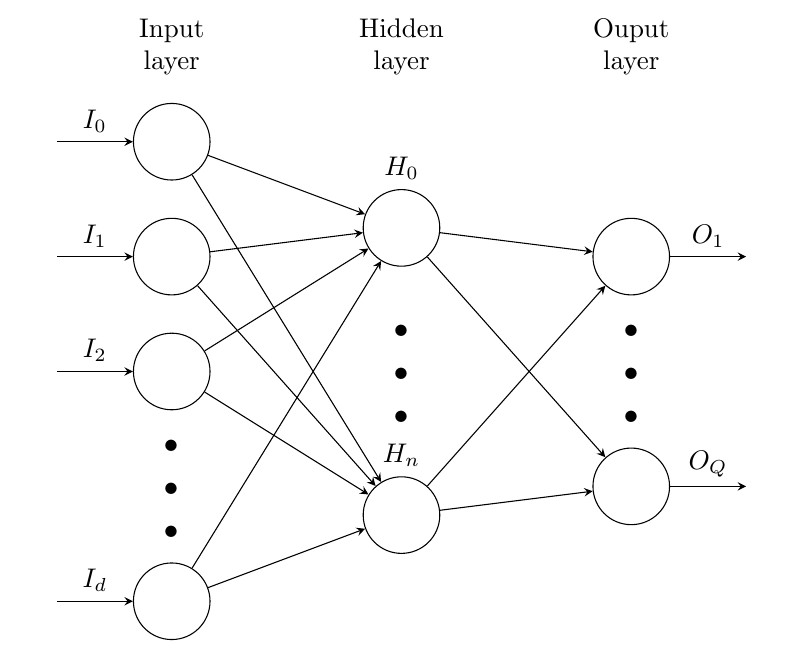
\includegraphics[width=0.8\textwidth]{MultiLabelNet.jpeg}
\caption{\label{fig:MultiLabelNet}Network Topology For Multi-lable classification}
\end{figure}

The network has $d$ input neurons which corresponds to a $d$-dimensional feature vector, while last $Q$ neurons represent a combination of output labels. There is a hidden layer in \ref{fig:MultiLabelNet} which owns $n$ hidden neurons. Input layer is fully connected with hidden layer and the same connecting method between hidden layer and output layer. So there are $d x n$ weights $(W_{ih}, 1 \leq i \leq d, 1 \leq h \leq n)$ between input layer and hidden layer and $n x q$ weights $(W_{ho}, 1 \leq h \leq n , 1 \leq o \leq q)$ between hidden layer and output layer. The bias parameters are represented as $I_{0}$ and  $H_{0}$.

Because the task of multi-label learning is to predict labels of test samples, it needs to evaluate the global error of model as:
\begin{equation}\label{eq:MultiLableError}
E = \sum_{i=1}^m E_{i}
\end{equation}
$E_{i}$ is the error on sample $x_{i}$ which can be defined as:
\begin{equation}\label{eq:MultiLableSamError}
E_{i} = \sum_{j=1}^Q (c_{j}^i - d_{j}^i)^2
\end{equation}
where $c_{j}^i = c_{j}(x_{i})$ is predicted $j$-th label by model on sample $x_{i}$, and $d_{j}^i$ is actual $j$-th label of sample $x_{i}$. The actual label has value of either $+1 (j \in mathcal{Y_{i}})$ or $-1 (j \notin mathcal{Y_{i}})$.

Various learning algorithms can be used to achieve a model based on training dataset. Backpropagation(BP) algorithm is deployed to learn from errors. However, original BP algorithm could be improper in multi-label learning because the error function\ref{eq:MultiLableSamError} neglects the correlations among labels of a sample. In original BP algorithm, the error function\ref{eq:MultiLableSamError} limits on individual label discrimination, such that a specific label $j \in mathcal{Y}$ belongs to sample $x_{i}$ or not. It should be taken into consider that labels in $Y_{i}$ is more important than those outside of $Y_{i}$. A new global error function is defined as:
\begin{equation}\label{eq:MultiLableGlobalError}
E = \sum_{i=1}^m E_{i} = \sum_{i=1}^m \frac{1}{|Y_{i}||\hat{Y}_{i}|} \sum_{(k,l) \in Y_{i} \times \hat{Y_{i}}} exp(-(c_{k}^i-c_{l}^i))
\end{equation}
In error function\ref{eq:MultiLableGlobalError}, $i$-th errors on the $i$-th multi-label training sample $(x_{i},Y_{i})$ have been accumulated. $\hat{Y}_{i}$ is complementary set of $Y_{i}$ in $\mathcal{Y}$ and $|\cdot|$ computes the cardinality of a set. 
Specifically, $c_{k}^i-c_{l}^i$ represents the difference between the output labels of network on a label which belongs to sample $x_{i}$ and a label which does not belong to the same sample. The error function\ref{eq:MultiLableGlobalError} shows that bigger difference leads to better performance. Additionally, the negation of the difference is put into the exponential function to sharply penalize the $i$-th term if $c_{k}^i$ is much smaller than $c_{l}^i$. The sum of $i$-th error term accumulates difference between outputs of any pair of labels of which one belongs to the sample and the other does not belong to it. The sum is normalized by the numbers of all pairs, $|Y_{i}||\hat{Y}_{i}|$. Then, the correlations between pair labels are computed. In the other words, labels in $Y_{i}$ should get larger output value than labels in $\hat{Y}_{i}$.

As previous statements, error function\ref{eq:MultiLableGlobalError} calculates the difference between output labels of which some belong to a sample and others do not belong to it. The task of learning is minimizing error function\ref{eq:MultiLableGlobalError} via enlarging output values of labels belonging to the training samples and diminishing output values of labels not belonging to it. If training dataset can cover the distribution of whole sample space, neural network model can learn it through minimizing error function by feeding training dataset.

\subsection{Error Function}

The basic goal of regression problems is to figure out the conditional distribution of the output labels, given the input samples. It is common to use a sum-of-squares error function.

The basic goal of classification problems is to figure out the posterior probabilities of class types, given the input samples. Except for sum-of-squares error function, there are some more approximate error functions which can be considered.

The central goal in training neural network is to model the hidden generator of the samples instead of memorizing the training samples. Therefore, the best prediction of an input sample can be found if the network can present a new value for the sample. Because the general and complete characterization of the generator of the dataset is the probability density $p(x,t)$. It is available to decompose a joint probability density into the product of the conditional density of the labels, the input data and the density of input data,
\begin{equation}\label{eq:JointProbDensity}
p(x,t) = p(t|x)p(x)
\end{equation}
where $p(t|x)$ represents the probability density of $t$ if $x$ is a distinct label and $p(x)$ represents the density of $x$
\begin{equation}\label{eq:ProbDensityX}
p(x) = \int p(t,x)dt
\end{equation}

Most error functions can be obtained from the idea of maximum likelihood. For training dataset, 
\begin{equation}\label{eq:LikelihoodLoss}
L = \coprod_{\substack{n}}  p(t^n|x^n)p(x^n)
\end{equation}
where each sample is picked out randomly from the same  distribution and their probabilities can be multiplied. The error function can be represented by minimizing the negative logarithm of the likelihood since the negative logarithm is a monotonic function.
\begin{equation}\label{eq:LikelihoodErrorFunc}
E = -ln L = -\sum_{\substack{n}} ln p(t^n|x^n) - \sum_{\substack{n}}lnp(x^n)
\end{equation}
where $E$ is notated as error function. The task of feed-forward neural network is to model the conditional probability density $p(t|x)$. And the second term is independent with the parameters in neural networks.  We can simplify \ref{eq:LikelihoodErrorFunc} to
\begin{equation}\label{eq:SimLikelihoodErrorFunc}
E = -ln L = -\sum_{\substack{n}} ln p(t^n|x^n) + C
\end{equation}
It is worth noting that error functions are dependent on different assumptions of the forms of the conditional distribution $p(t|x)$. In this classification task, $t$ represents labels which act as class members or the prediction of the probabilities of class members.

\subsection{Cross Entropy}

The Mean Square Error is a common risk metric comparable to the predicted value of the squared error loss. It is simple to implementation and non-negative. However, it has the disadvantage of heavily weighting outliers\citep{bermejo2001oriented}.

Given that there are two discrete distributions $p(x)$ and $q(x)$ over the same variable $x$. The relative entropy, relating to cross entropy, is a method to measure the distance between the distributions:
\begin{equation}\label{eq:RelativeEngtropy}
D_{pq}(p(x), q(x)) = \sum_{\substack{x}}q(x)ln\frac{q(x)}{p(x)}
\end{equation}
where the relative entropy is not a true metric because \ref{eq:RelativeEngtropy} could not be symmetric in the interchange $p \leftrightarrow q$ and probably not satisfy the triangle inequality.

Cross entropy loss, also called logistic regression loss, is an alternative method of estimating probability distributions. The measure is commonly used in neural networks. It can be used to evaluate the posterior probabilities of class membership.




\subsection{Training and Testing}

Following previous process, gradient descent is used to minimize the global error function with backpropagation. 

To train a sample $(x_{i}, Y_{i})$,in while $x_{i}$ is input data and $Y_{i}$ is associated label, the predicted output labels computed by neural network for is
\begin{equation}\label{eq:MultiLabelActivation}
c_{k} = f(netc_{k} + \theta_{k})
\end{equation}
where $\theta_{k}$ is the bias units of $k$ layer, $f()$ is the activation function of the output neurons which is a $tanh$ function\ref{eq:tanh} in this project. $netc_{k}$ is the input data of the layer:
\begin{equation}\label{eq:MultiLabel}
netc_{k} = \sum_{s=1}^M b_{s}w_{sk}
\end{equation}
where $w_{sk}$ is the weights connecting layer $s$ and $k$, while $M$ is the number of neurons in the hidden layer.

As $tanh$ function is differentiable, the general error of the $k$-th output neuron can be defined as:
\begin{equation}\label{eq:MultiLableErrorDif}
d_{k} = -\frac{\partial E}{\partial netc_{k}}
\end{equation}
combining with \ref{eq:MultiLabelActivation}, we can get
\begin{equation}\label{eq:MultiLableChainRule}
d_{k} = -\frac{\partial E_{i}}{\partial c_{j}} \frac{\partial c_{j}}{\partial netc_{k}} = - \frac{\partial E_{i}}{\partial c_{j}} f'(netc_{k} + \theta_{k})
\end{equation}
With considering global error function \ref{eq:MultiLableGlobalError}
\begin{equation}\label{eq:MultiLablePartialC}
\frac{\partial E_{i}}{\partial c_{j}}= 
\begin{cases}
    -\frac{1}{|Y_{i}||\hat{Y}_{i}|} \sum_{l \in \hat{Y}_{i}} exp(-(c_{j} - c_{l}))       & \quad \text{if } j \in Y_{i}\\
    \frac{1}{|Y_{i}||\hat{Y}_{i}|} \sum_{k \in Y_{i}} exp(-(c_{k} - c_{j}))       & \quad \text{if } j \in \hat{Y}_{i}\\
  \end{cases}
\end{equation}
with derivation of $tanh$, and substituting it with \ref{eq:MultiLableChainRule} and \ref{eq:MultiLablePartialC} we can get
\begin{equation}\label{eq:MultiLableGenErr}
d_{k}= 
\begin{cases}
    \big(-\frac{1}{|Y_{i}||\hat{Y}_{i}|} \sum_{l \in \hat{Y}_{i}} exp(-(c_{j} - c_{l}))\big)(1+c_{j})(1-c_{j})       & \quad \text{if } j \in Y_{i}\\
    \big(\frac{1}{|Y_{i}||\hat{Y}_{i}|} \sum_{k \in Y_{i}} exp(-(c_{k} - c_{j}))\big)(1+c_{j})(1-c_{j})       & \quad \text{if } j \in \hat{Y}_{i}\\
  \end{cases}
\end{equation}
According to previous method, we can define the general error of the $s$-th hidden neuron as:
\begin{equation}\label{eq:MultiLableGenErrS}
e_{s} = - \frac{\partial E_{i}}{\partial netb_{s}}
\end{equation}
with $b_{s} = f(netb_{s} + \lambda_{s})$ and chain rule,
\begin{equation}\label{eq:MultiLablePartialE}
e_{s} = - \frac{\partial E_{i}}{\partial b_{s}} \frac{\partial b_{s}}{\partial netb_{s}} = - \big( \sum_{j=1}^Q \frac{\partial E_{i}}{\partial netc_{j}} \frac{\partial netc_{j}}{\partial b_{s}}\big)f'(netb_{s} + \lambda_{s})
\end{equation}
For $d_{j} = - \frac{\partial E_{i}}{\partial netc_{j}}$ and $netc_{j} = \sum_{s=1}^M b_{s}w_{sj}$, then 
\begin{equation}\label{eq:MultiLableGenErrEs}
e_{s} = \big( \sum_{j=1}^Q d_{j} \times \frac{\partial (\sum_{s=1}^M b_{s}w_{sj})}{\partial b_{s}}\big) f'(netb_{s} + \lambda_{s}) = \big( \sum_{j=1}^Q d_{j}w_{sj}\big) f'(netb_{s} + \lambda_{s})
\end{equation}
As function $f()$ is $tanh$, we get
\begin{equation}\label{eq:MultiLableGenErrEsFin}
e_{s} = \big( \sum_{j=1}^Q d_{j}w_{sj}\big) (1+b_{s})(1-b_{s})
\end{equation}
Stochastic gradient descent(SGD) method is used to approximate function.
\begin{equation}\label{eq:MultiLableUpdateWeights}
\Delta w_{sj} = -\alpha \frac{\partial E_{i}}{\partial w_{sj}} = \alpha \frac{\partial E_{i}}{\partial netc_{j}} \frac{\partial netc_{j}}{\partial w_{sj}} = \alpha d_{j}b_{s}
\end{equation}
\begin{equation}\label{eq:MultiLableUpdateHidWeights}
\Delta v_{hs} = -\alpha \frac{\partial E_{i}}{\partial v_{hs}} = \alpha \frac{\partial E_{i}}{\partial netb_{s}} \frac{\partial netb_{s}}{\partial v_{hs}} = \alpha e_{s}a_{h}
\end{equation}
while bias are updated according to
\begin{equation}\label{eq:MultiLableUpdateBias}
\Delta \theta_{j} = \alpha d_{j} \text{ } \Delta \lambda_{s} = \alpha e_{s}
\end{equation}
in previous Equations, $\alpha$ is learning rate in the range of $[0.0 \text{ } 1.0]$.

Based on previous process, a learning algorithm has been set up with backpropagation. More ever, training samples are fed into neural network in each epoch. After all training samples $((x, Y)$ fed into network, weights and bias are updated through equations\ref{eq:MultiLableUpdateWeights} and \ref{eq:MultiLableUpdateBias}. The training samples are fed into the network iteratively while global error value decreases. Finally, the error value converge to a minimum value.

In testing process, network predicts a sample which has a set of actual labels $c_{j} (j = 1,2,...,Q)$ by ranking the labels. Because the output values of each label is in range $[-1.0,1.0]$, a threshold function $t(x)$ is used to determine associated label set for the sample $x$. A large margin ranking system\citep{elisseeff2001kernel} is adopted to generalize the sets. $t(x)$ is a linear function, $t(x) = w^T\cdot c(x) + b$, where $c(x) = (c_{1}(x), c_{2}(x),...,c_{Q}(x))$ is a $Q$-dimensional vector which represent $j$ output labels of a sample. Learning the threshold function $t(x)$ follows the next steps. For every training sample $(x_{i}, Y_{i}) (1 \leq i \leq m)$, the relation between $c(x_{i})$ and target value $t(x_{i})$ is:
\begin{equation}\label{eq:MultiLableThreshFunc}
t(x_{i}) =  \operatorname{arg\,max}_t (|\{k|k \in Y_{i}, c_{k}^i \leq t\}| + |\{l|l \in \hat{Y}_{i}, c_{l}^i \geq t\}|) 
\end{equation}
If there are several minimum values and optimal values are in a division, the middle value of the division is chosen. The task of learning the parameters of threshold function is to solve the matrix equation $\Phi \cdot w' = t$. The matrix $\Phi$ has dimensions $m \times (Q + 1)$ in which $i$-th vector is $(c_{1}^i, c_{2}^2,...,c_{Q}^i,1)$, $w'$ is $(Q+1)$ dimensional vector $(w,b)$ and $t$ is the $m$ dimensional vector $(t(x_{1}), t(x_{2}),...,t(x_{m}))$. Linear least squares is used to find the solution of the equation. Given a sample $x$, the network predicts output label vector $c(x)$ and the threshold value for $x$ is gotten by solving equation$t(x) = w^T \cdot c(x) + b$.

The computation complexity of evaluating derivatives of the error function is linearly with neuron size of network. Three main components are composed of computation, feedforward process, backpropagation process and updating weights process. In feedforward process to compute $b_{i}$ and $c_{j}$, the computation cost is mainly on evaluation the sums and activation function. In backpropagation process(\ref{eq:MultiLableGenErr}and\ref{eq:MultiLableGenErrEsFin}), the computation complexity of $d_{k}$ and $e_{s}$ is $O(Q)$. In updating weights process, the overall computational cost is $O(W)$ where $W$ is the total number of weights . 

